\section*{Problem 2 - Attitude Control using Euler Angles}
\subsection*{Problem 2.1}
The Lyapunov function candidate and the PD-controller can be written as 

\begin{equation}
\label{eq:yes}
	V &= \frac{1}{2} \boldsymbol{\omega}^{\top} \mathbf{I}_{CG} \boldsymbol{\omega} + \frac{1}{2} \tilde{\boldsymbol{\Theta}}^{\top} \mathbf{K}_p \boldsymbol{\tilde{\Theta}}
\end{equation}

\begin{equation}\label{eq:insert}
\boldsymbol{\tau} &= -\mathbf{K}_d \boldsymbol{\omega} -\mathbf{T}_{\Theta}^{\top}(\Theta) \mathbf{K}_p \tilde{\boldsymbol{\Theta}}
\end{equation}


Since $\boldsymbol{I}_{CG}$, $\boldsymbol{K}_d$ and $\boldsymbol{K}_p$ are symmetric, $\dot{V}$ becomes
\begin{equation} \label{eq:as}
\dot{V} = \boldsymbol{\omega}^T\boldsymbol{I}_{CG}\dot{\boldsymbol{\omega}} + \tilde{\boldsymbol{\Theta}}^T\boldsymbol{K}_p\boldsymbol{\dot{\Theta}}
\end{equation}

Inserting  (\ref{eq:kinetics}) into (\ref{eq:as})

\begin{equation}\label{eq:into}
\dot{V} = \boldsymbol{\omega}^T\left( \boldsymbol{\tau} + (\boldsymbol{I}_{CG}\boldsymbol{\omega})\times \boldsymbol{\omega} \right) + \tilde{\boldsymbol{\Theta}}^T\boldsymbol{K}_p\boldsymbol{\dot{\Theta}}
\end{equation}

and inserting (\ref{eq:insert}) into (\ref{eq:into})

\begin{equation}
\dot{V} = \boldsymbol{\omega}^T\left(  -\mathbf{K}_d \boldsymbol{\omega} -\mathbf{T}_{\Theta}^{\top}(\Theta) \mathbf{K}_p \tilde{\boldsymbol{\Theta}} + (\boldsymbol{I}_{CG}\boldsymbol{\omega})\times \boldsymbol{\omega} \right) + \tilde{\boldsymbol{\Theta}}^T\boldsymbol{K}_p\boldsymbol{\dot{\Theta}}
\end{equation}

From equation (\ref{eq:see}) we know that $\mathbf{T}_{\Theta}(\Theta)\boldsymbol{\omega} =\boldsymbol{\dot{\Theta}}$

\begin{equation}
\begin{align}
    \dot{V} &=   -\boldsymbol{\omega}^T\mathbf{K}_d \boldsymbol{\omega} -\boldsymbol{\omega}^T\mathbf{T}_{\Theta}^{\top}(\Theta) \mathbf{K}_p \tilde{\boldsymbol{\Theta}} + \boldsymbol{\omega}^T(\boldsymbol{I}_{CG}\boldsymbol{\omega})\times \boldsymbol{\omega}  + \tilde{\boldsymbol{\Theta}}^T\boldsymbol{K}_p\boldsymbol{\dot{\Theta}}\\
    &= -\boldsymbol{\omega}^T\mathbf{K}_d \boldsymbol{\omega} - \cancel{\dot{\boldsymbol{\Theta}} \boldsymbol{K}_p \tilde{\boldsymbol{\Theta}}} + \boldsymbol{\omega}^T(\boldsymbol{I}_{CG}\boldsymbol{\omega})\times \boldsymbol{\omega}  + \cancel{\tilde{\boldsymbol{\Theta}}^T\boldsymbol{K}_p\boldsymbol{\dot{\Theta}}}\\
    &=-\boldsymbol{\omega}^T\mathbf{K}_d \boldsymbol{\omega} + \boldsymbol{\omega}^T(\boldsymbol{I}_{CG}\boldsymbol{\omega})\times \boldsymbol{\omega}\\
    &= -\boldsymbol{\omega}^T\mathbf{K}_d \boldsymbol{\omega} + (\boldsymbol{I}_{CG}\boldsymbol{\omega})^T\boldsymbol{\omega}\times \boldsymbol{\omega}
     \\&=-\boldsymbol{\omega}^T\mathbf{K}_d \boldsymbol{\omega}
\end{align}
\end{equation}

For a function to be a Lyapunov function it must satisfy $V(x)>0$ and $\dot{V}(x)\le 0$. Therefore, $\boldsymbol{K}_p>0$ and $\boldsymbol{K}_d > 0$ 

\subsection*{Problem 2.2}

If we assume that $V$ is a true Lyapunov function candidate we know that \\$V(t)\le V(0)$ and $\dot{V} \le 0$. This means that $\boldsymbol{\omega}$ must be bounded. If we calculate the second derivative of $V$ we get $\ddot{V} = -\boldsymbol{K_d\omega}< 0$, since $\boldsymbol{\omega}$ is bounded, $\dot{V}$ converges, and therefore $\boldsymbol{\omega}$ must converge.
I can't say anything about the error $\boldsymbol{\tilde{\Theta}}$ %since it is not in $\dot{V}$. 

\subsection*{Problem 2.3}
The set $\Omega$ is found by setting $\dot{V}=0$. $\dot{V}$ is zero when $\omega = 0$. $\Omega$ is then 
\begin{equation}
\Omega = \{ (x\epsilon \mathbb{R},\boldsymbol{\omega}=0) \}
\end{equation}

this means that

\begin{equation}
\boldsymbol{I}_{CG}\dot{\boldsymbol{\omega}} = -\boldsymbol{T}_{\Theta}^T(\Theta)\boldsymbol{K}_p\tilde{\boldsymbol{\Theta}}
\end{equation}

which means that $\tilde{\boldsymbol{\Theta}}= \boldsymbol{\Theta}- \boldsymbol{\Theta}_d = 0$,
from this we now know that the equilibrium point is $(\boldsymbol{\omega},\boldsymbol{\Theta}) = (0,\boldsymbol{\Theta_d})$, which are the only point in the largest set in $\Omega$. The point is GAS. 

\subsection*{Problem 2.4}
%Answer Problem 2.4 here. Figures can be inserted as:
%\begin{figure}[ht]
%	\centering
%	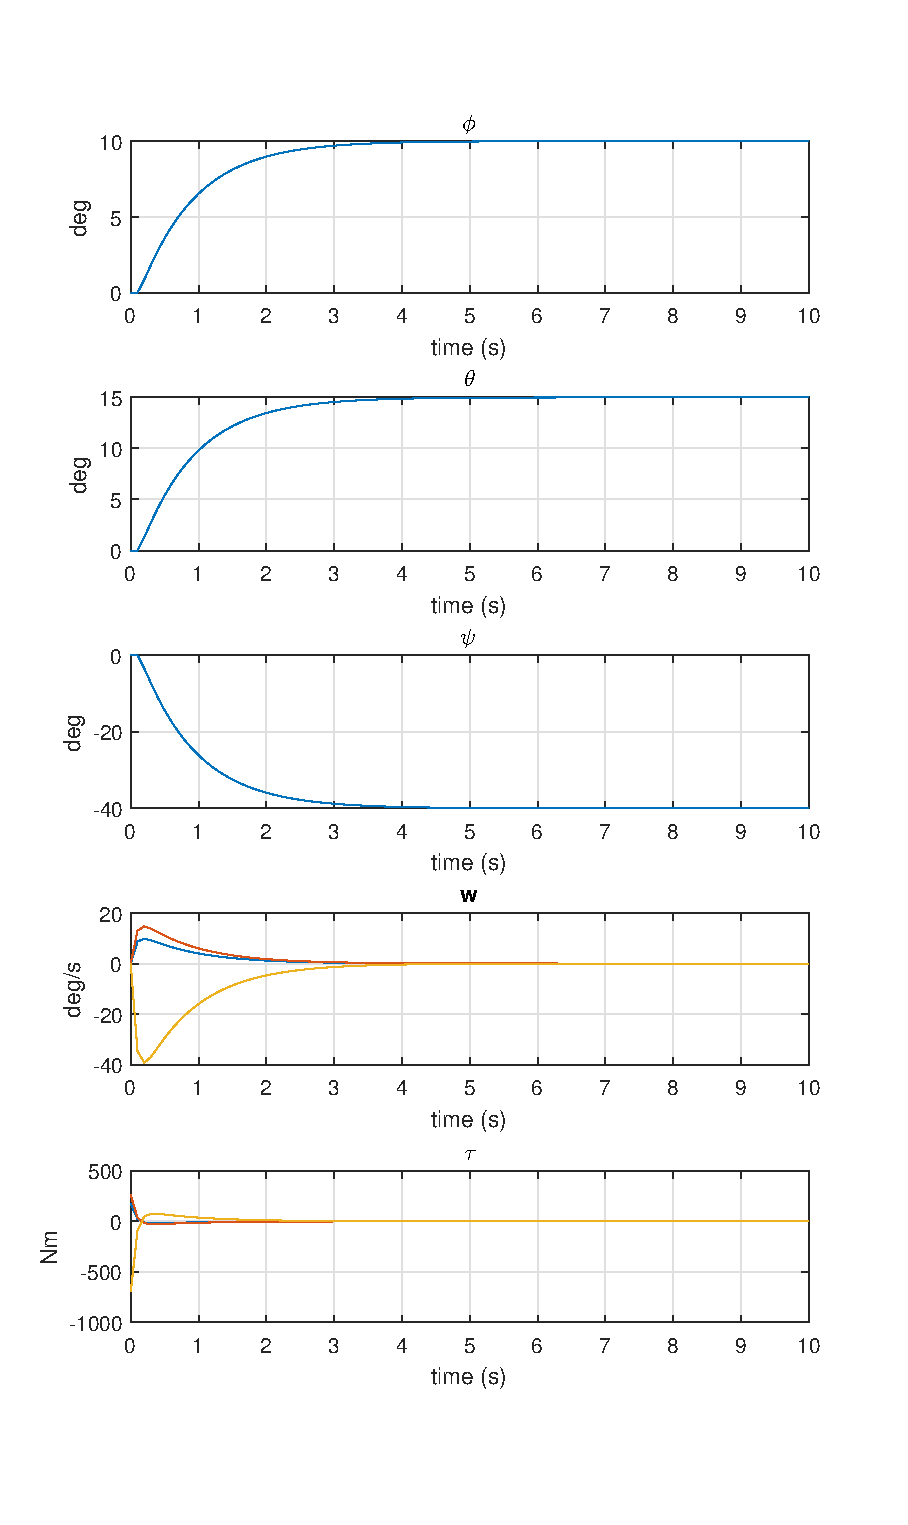
\includegraphics[width=0.7\textwidth]{1000eulerangles} % Filename is "fig1.png" and must be located in the same folder as this file. 
%	\caption{Figure of something useful.}
%	\label{fig:fig1}
%\end{figure}


\begin{figure}[ht]
	 \caption{We can see here that when we are close enough to zero, the system is easy to control, but when we set the initial $\theta$ to more than $60^\circ$ we are starting to get unwanted behavior. This is because of the singularity in $\theta = 90^\circ$}\label{fig:2}
	\centering
	\begin{subfigure}[b]{0.40\textwidth}
		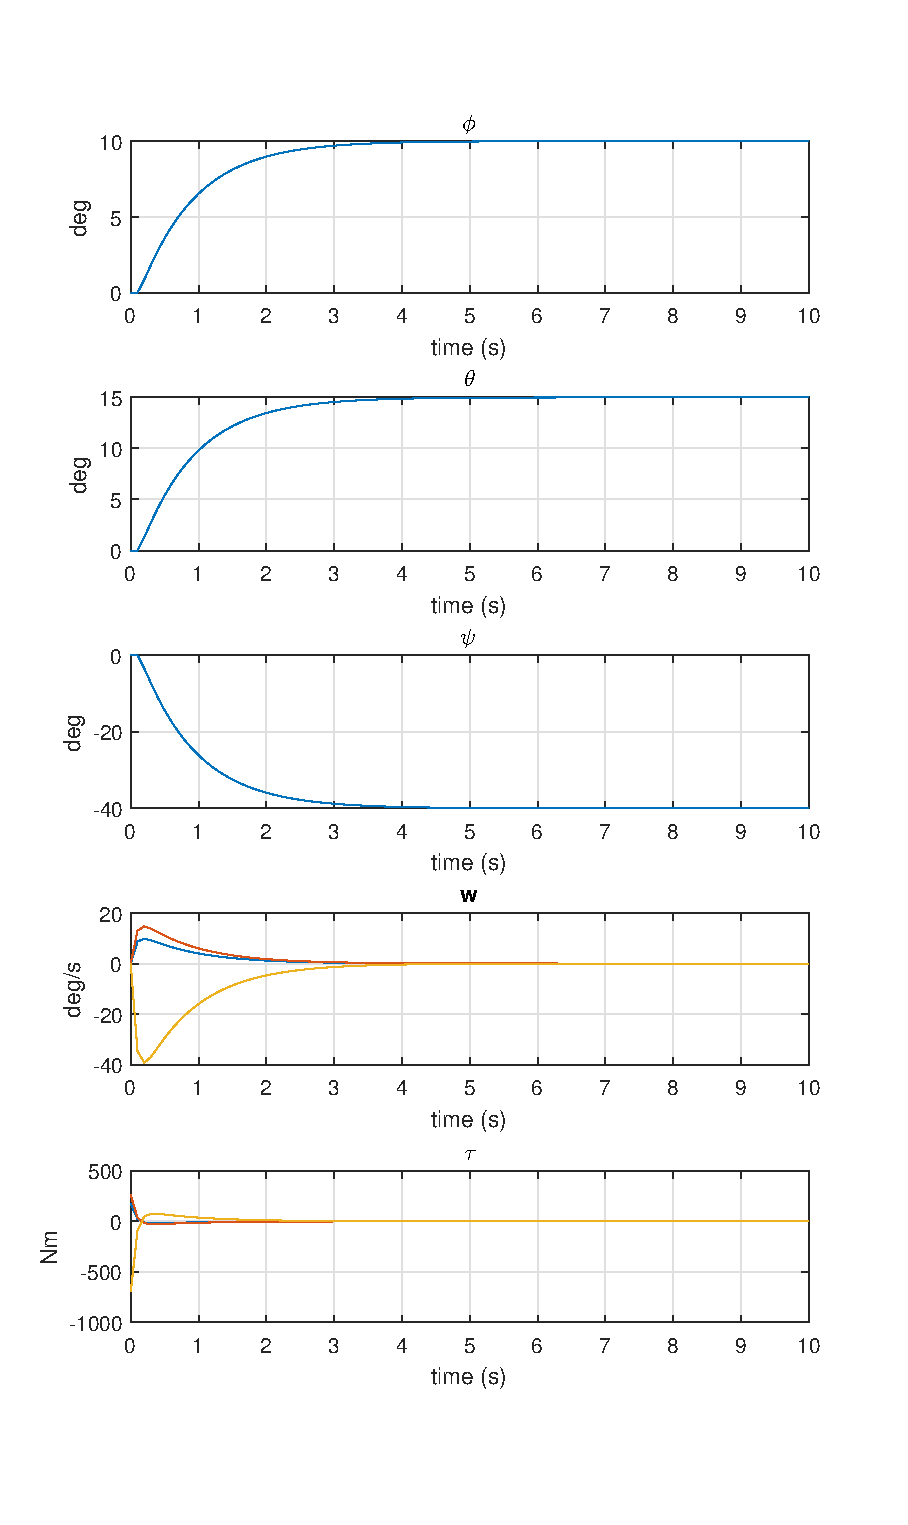
\includegraphics[width=\textwidth]{1000eulerangles}
		\caption{Here is a plot where the initial angles are zero and $\boldsymbol{K}_d = \boldsymbol{K}_p=1000\boldsymbol{I}_{3\times 3}$}
		\label{fig:2a}
	\end{subfigure}
	~ %add desired spacing between images, e. g. ~, \quad, \qquad, \hfill etc. 
	%(or a blank line to force the subfigure onto a new line)
	\begin{subfigure}[b]{0.40\textwidth}
		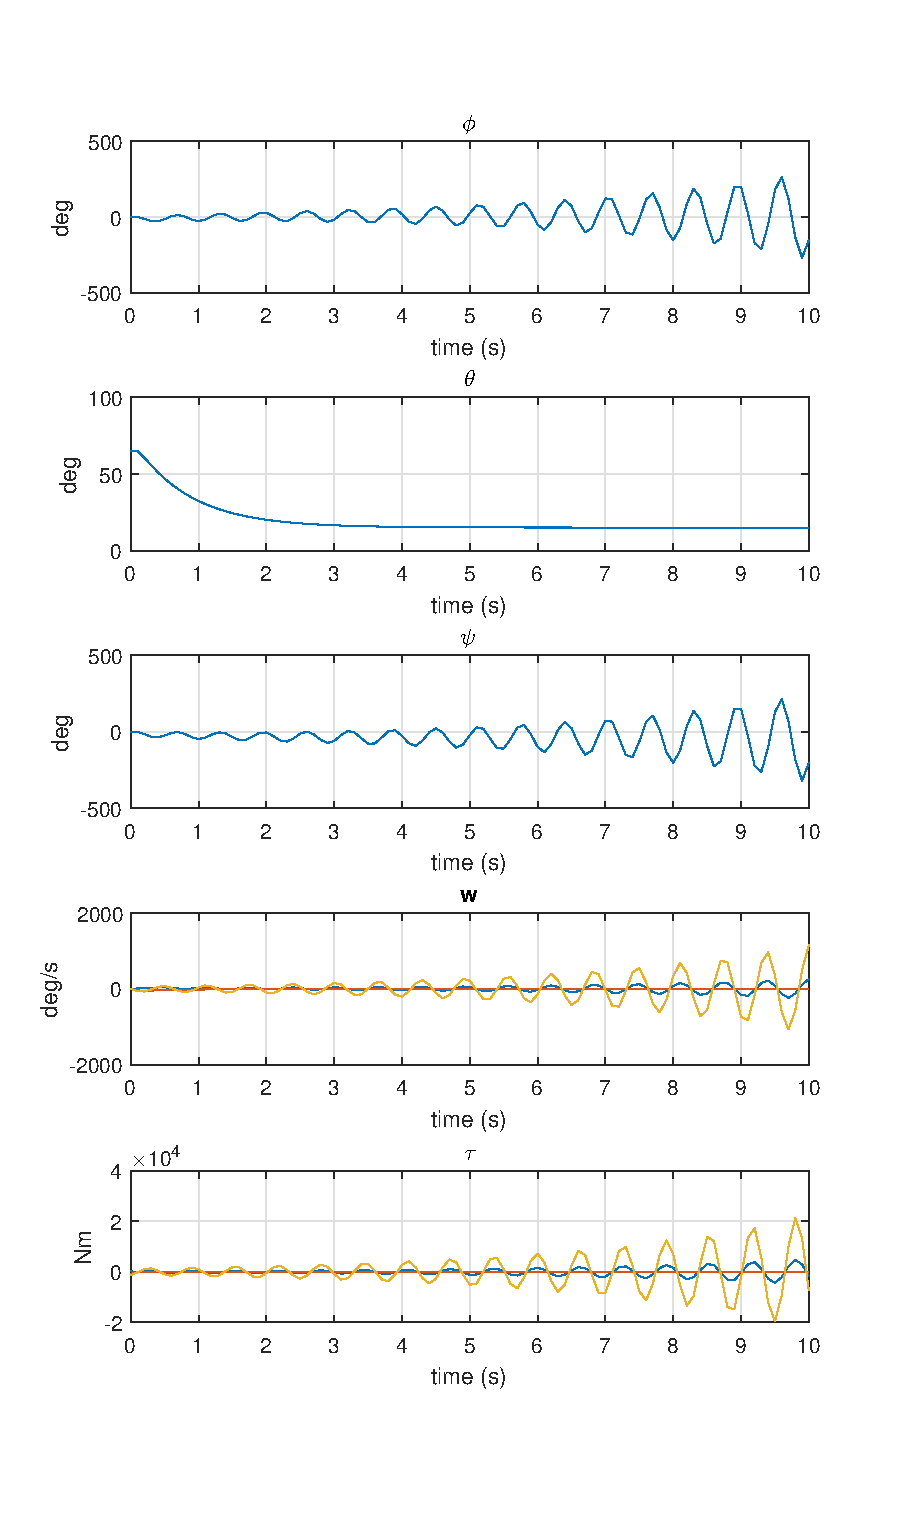
\includegraphics[width=\textwidth]{1000euleranglesunstable}
		\caption{In this plot the same $\boldsymbol{K_d}$ and $\boldsymbol{K_p}$ is used, but $\theta=65^\circ$ and the two other angles are zero}
		\label{fig:2b}
	\end{subfigure}
\end{figure}